\chapter{Results}
\label{ch:grundlagen}

Wichtige Info: Als Compiler muss \textbf{LuaLaTeX} verwendet werden. Auch in ShareLatex!

\section{Effectiveness Analysis}

[reword later]

is SURF IA less effective on certain runway geometries or not?

is SURF 
\section{Runway Incursions Distribution}
After thorough analysis of collected data, it was discovered, that vast majority of reported Runway Incursions happens in the United States (figure 4.1). Such strong concentration, might be due to cultural differences between countries on a topic of incident reporting. Relevant cases are shown on figure 4.2

\begin{figure} [H]
    \centering
    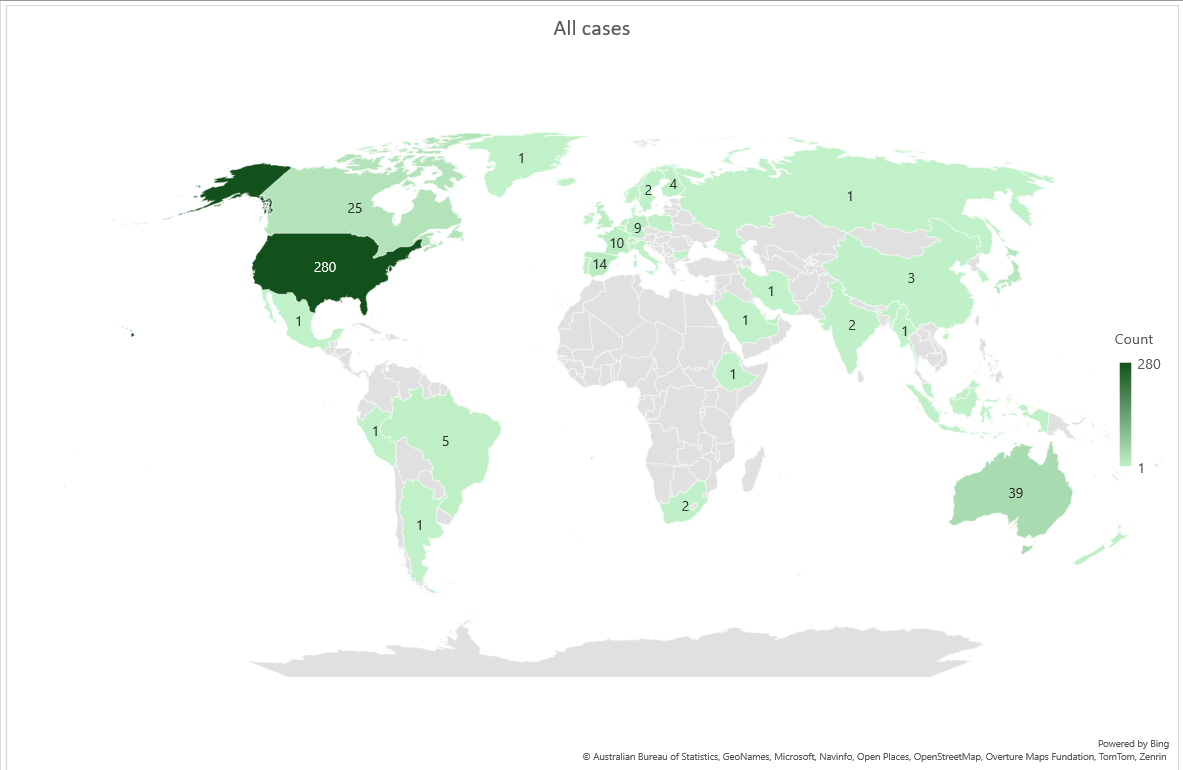
\includegraphics[width=0.9\linewidth]{Abbildungen/Geo_All.png}
    \caption{Geography of all incidents and accidents}
    \label{fig:enter-label}
\end{figure}

\begin{figure} [H]
    \centering
    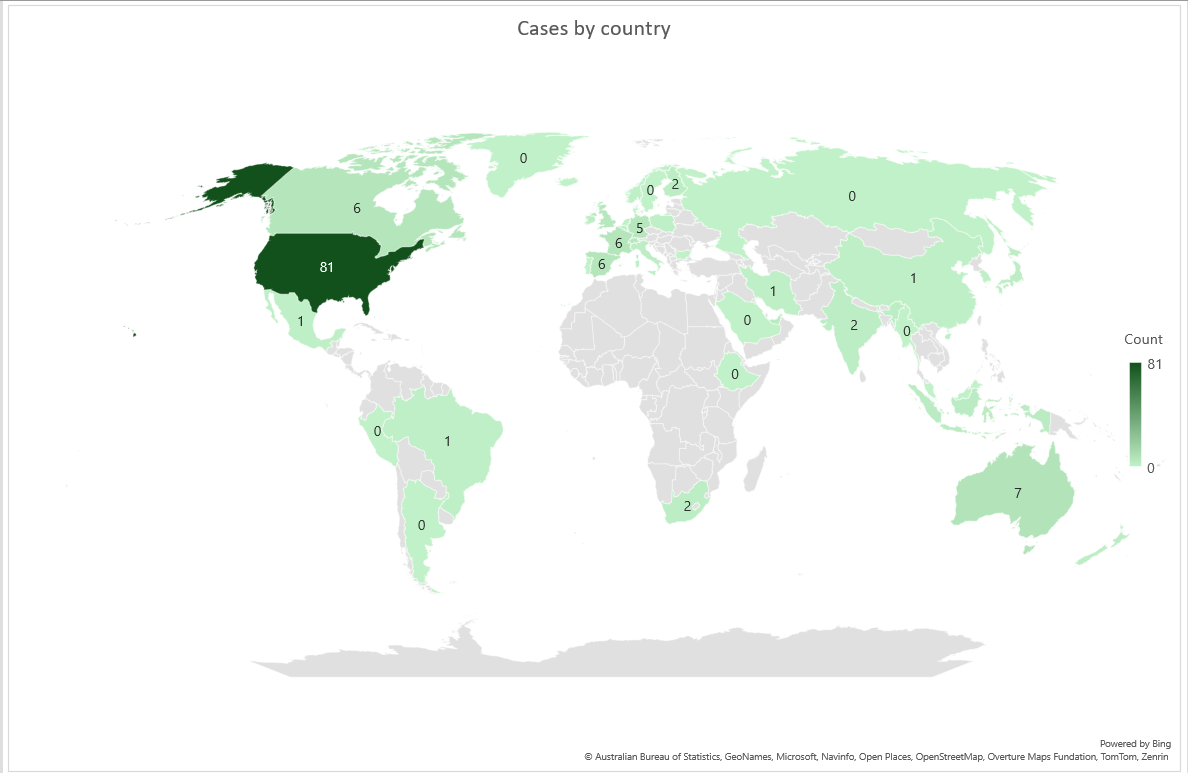
\includegraphics[width=0.9\linewidth]{Abbildungen/Geo_Relevant.png}
    \caption{Geography of relevant incidents and accidents}
    \label{fig:enter-label}
\end{figure}

 
\section{Analysis of Runway Incursions} 
It was discovered, that there are similar trends in runway incursions for both commercial and general aviation (figure 4.2). Although, it must be said, that the number of commercial cases in reality is higher, and number of cases is reduced due to strict filters for relevant cases for commercial aviation.

\begin{figure} [H]
        \centering
        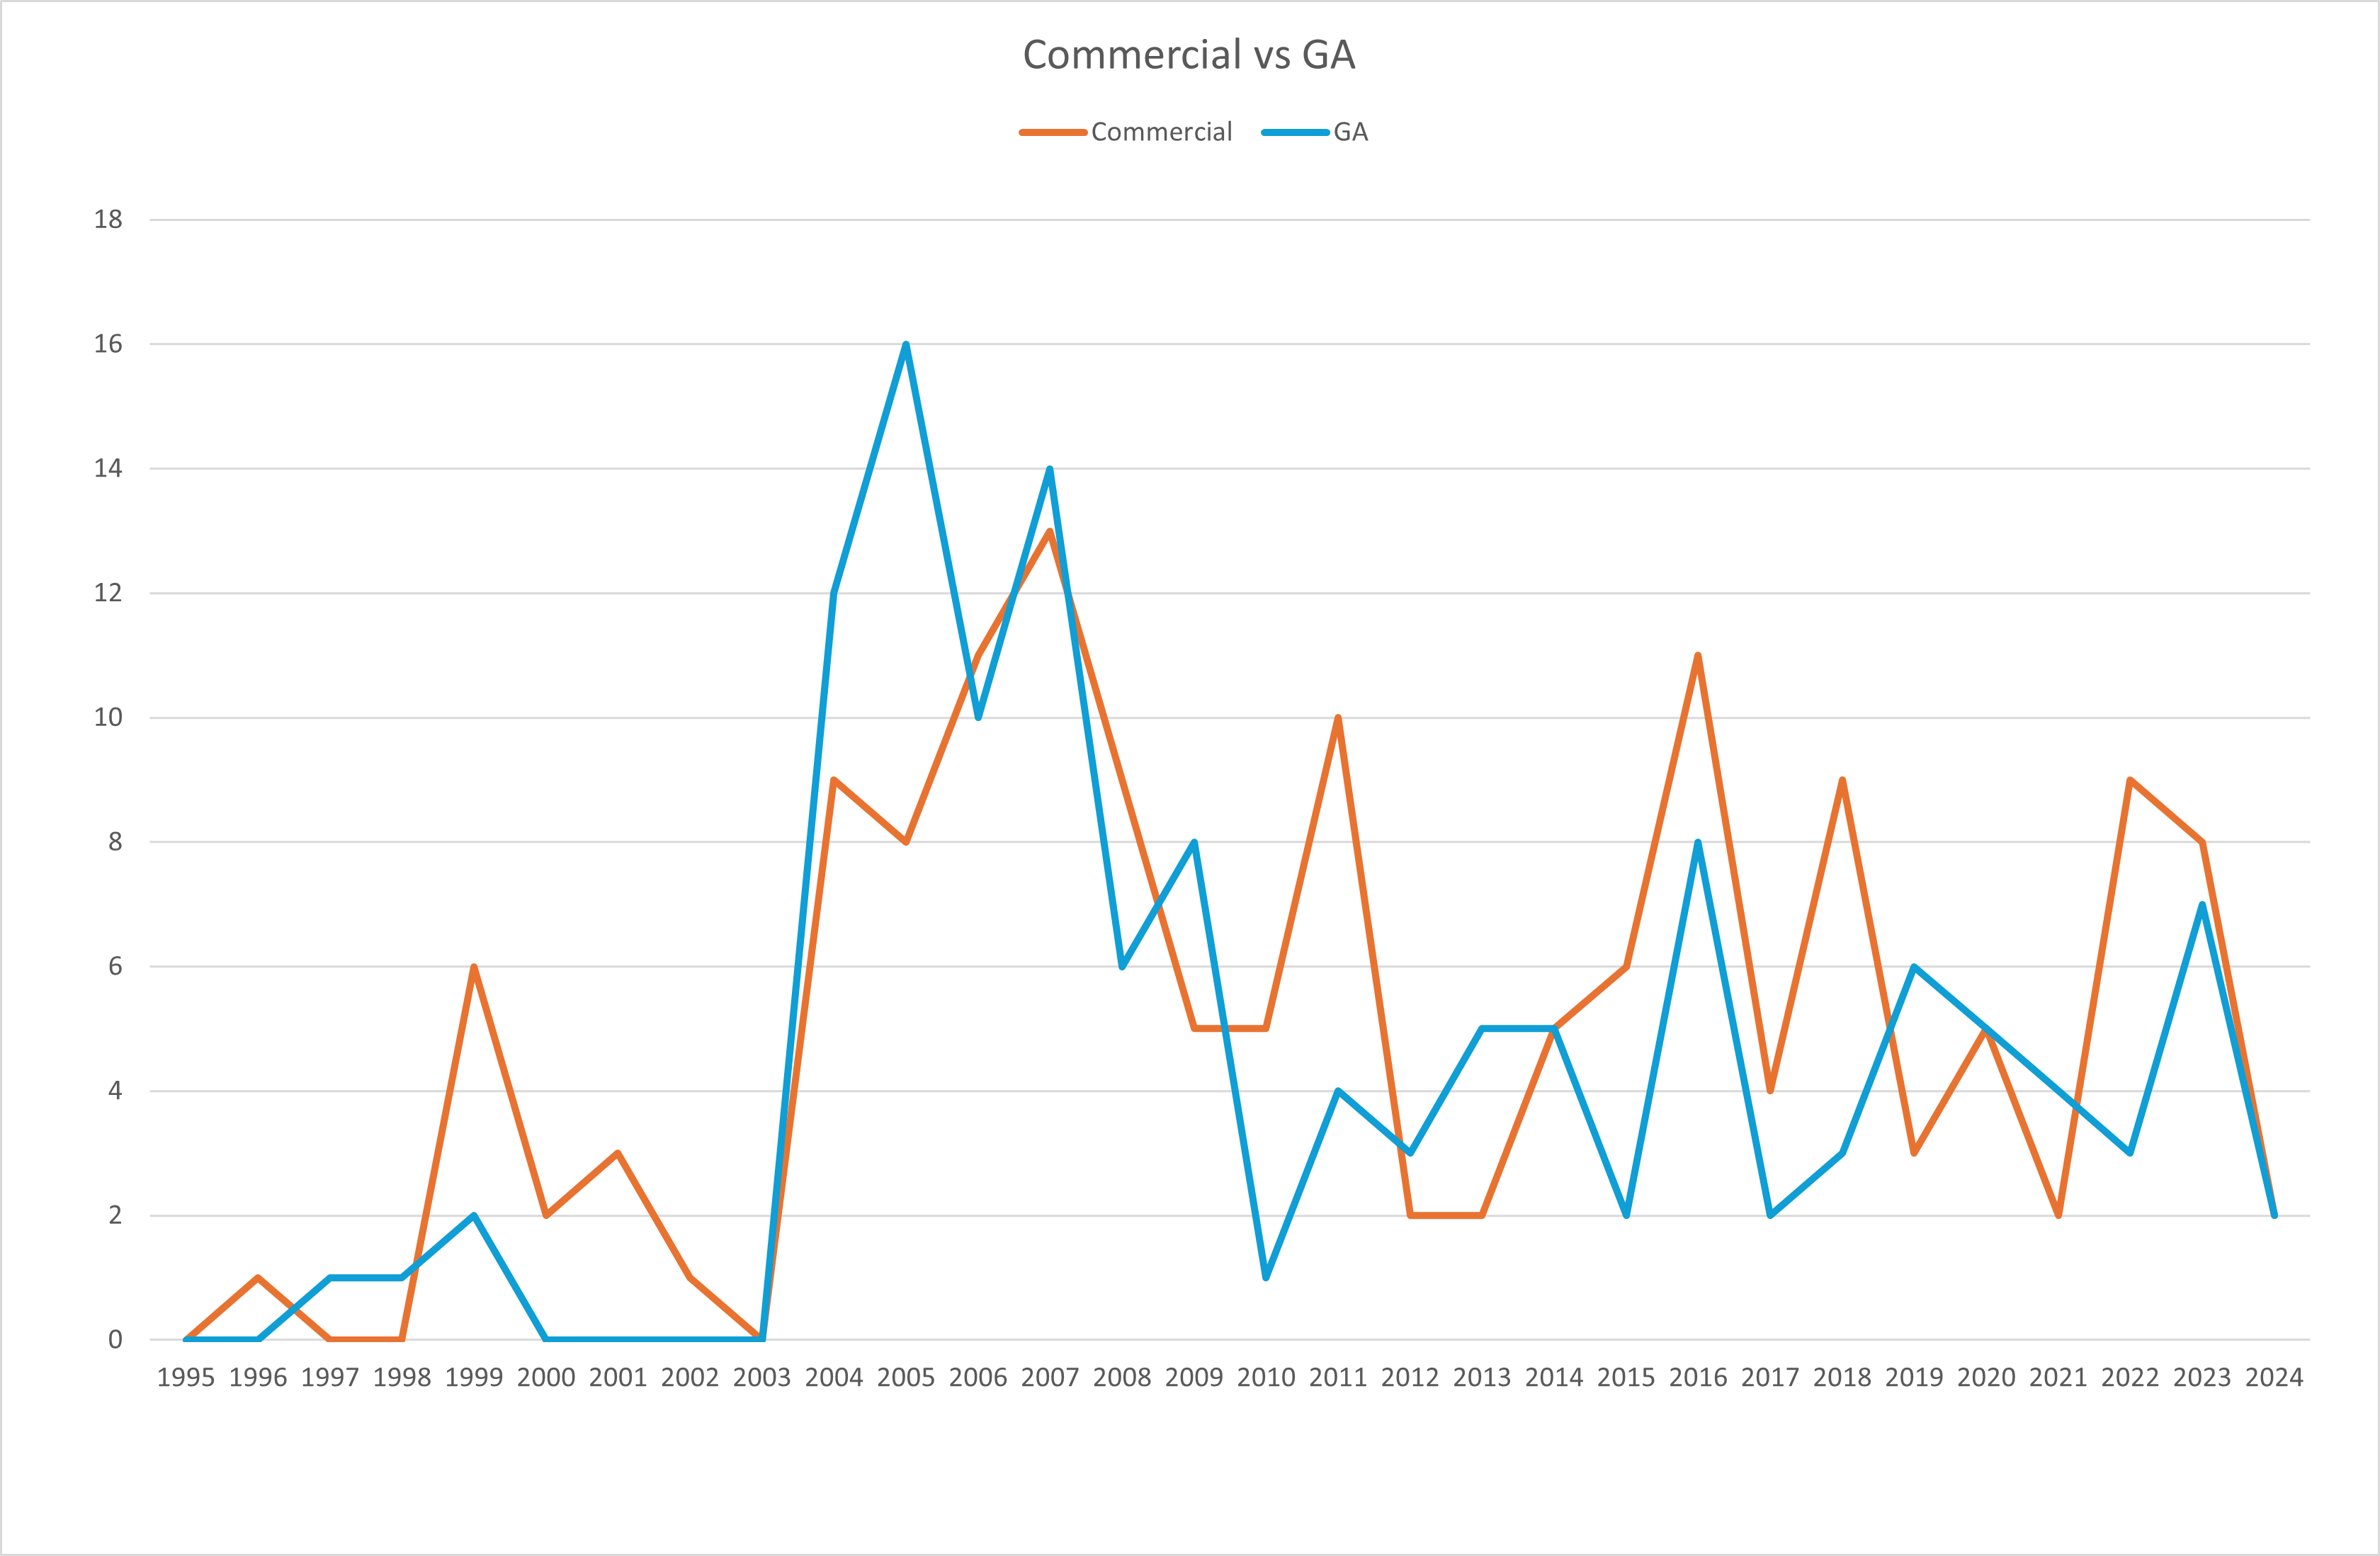
\includegraphics[width=0.75\linewidth]{Commercial_vs_GA_year.png}
        \caption{Commercial and GA year by year}
        \label{fig:enter-label}
\end{figure}


show frequency distribution graphs of category a and b runway incursions and effectiveness of SURF vs different parameters (runway geometry, cause, ownship and target type?. runway geometry for sure, still need to discuss about other parameters) discuss. try to find SURF detection logic reasoning for less effective detections vs others regarding conflict geometry

More than a half of the incidents were caused due to ATC error, or Operational Error (OE). While the other half was caused by Pilot Deviation (PD) or Pedestrian/Vehicle Deviation (P/VD).
\begin{figure} [H]
    \centering
    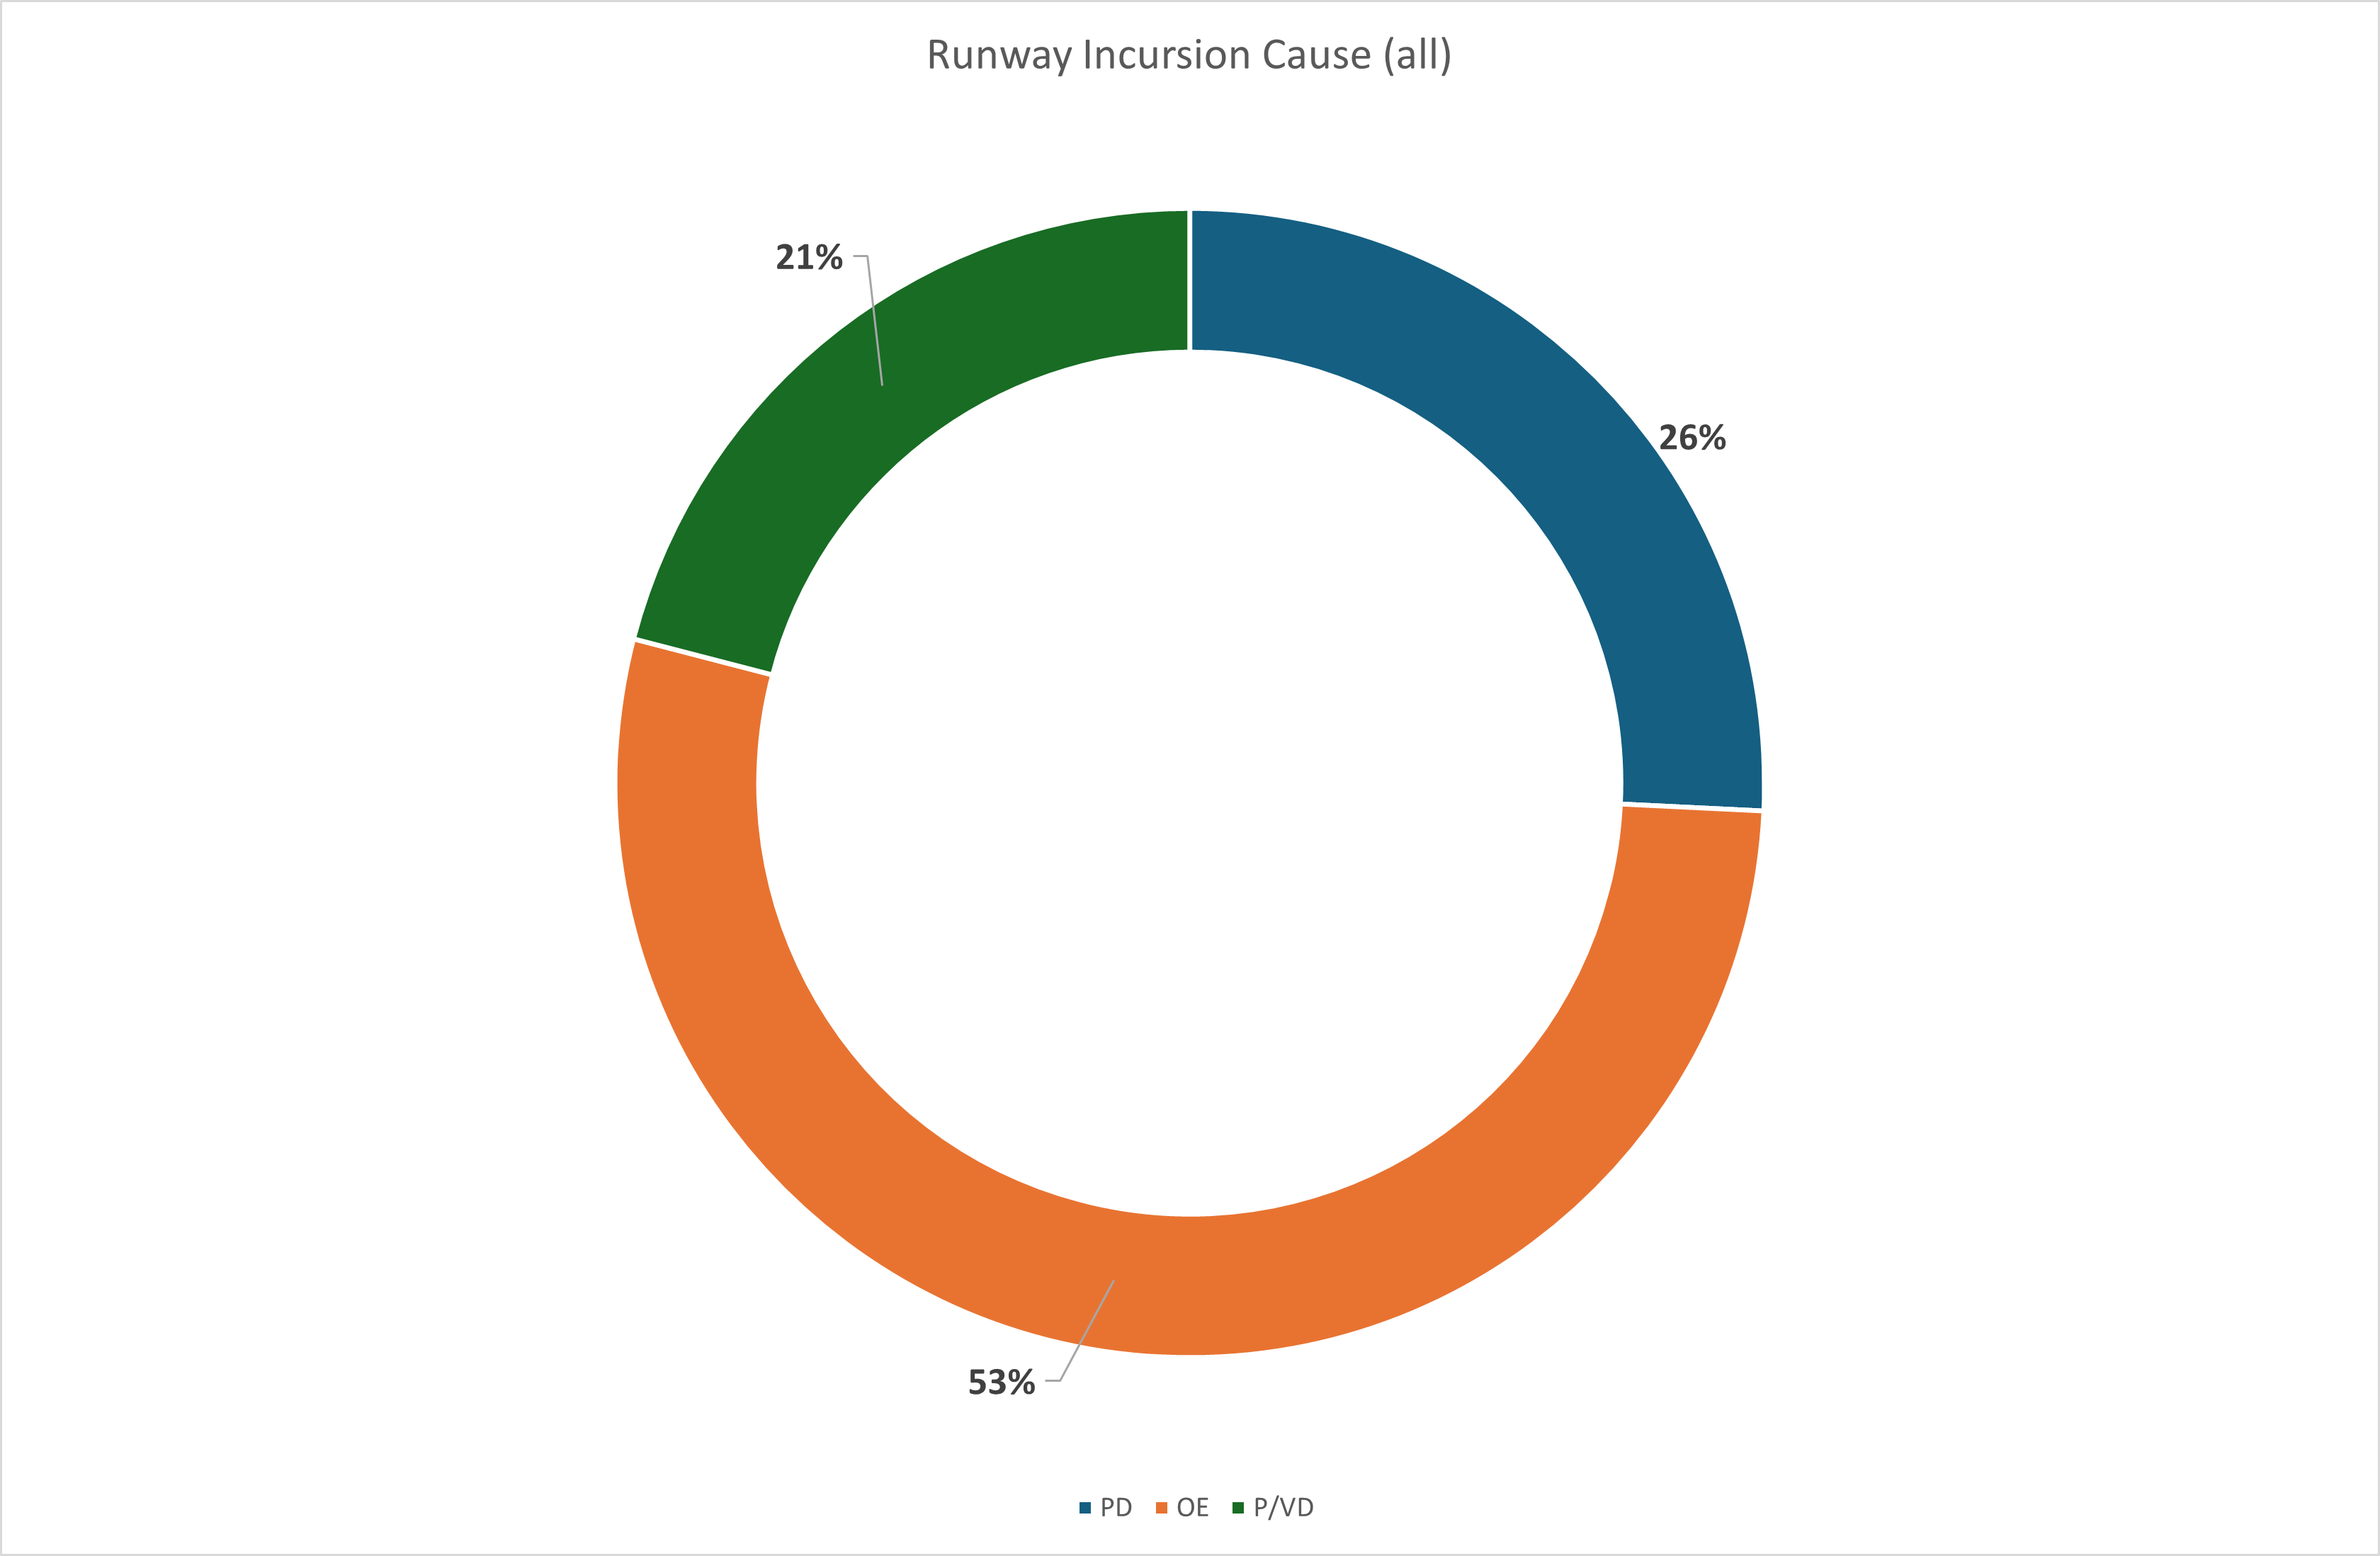
\includegraphics[width=0.75\linewidth]{Abbildungen/Cause_All.png}
    \caption{Cause All}
    \label{fig:enter-label}
\end{figure}

While in cases, that adhere to provided parameters - proportion is roughly 1 to 1 between PD and OE.
\begin{figure} [H]
    \centering
    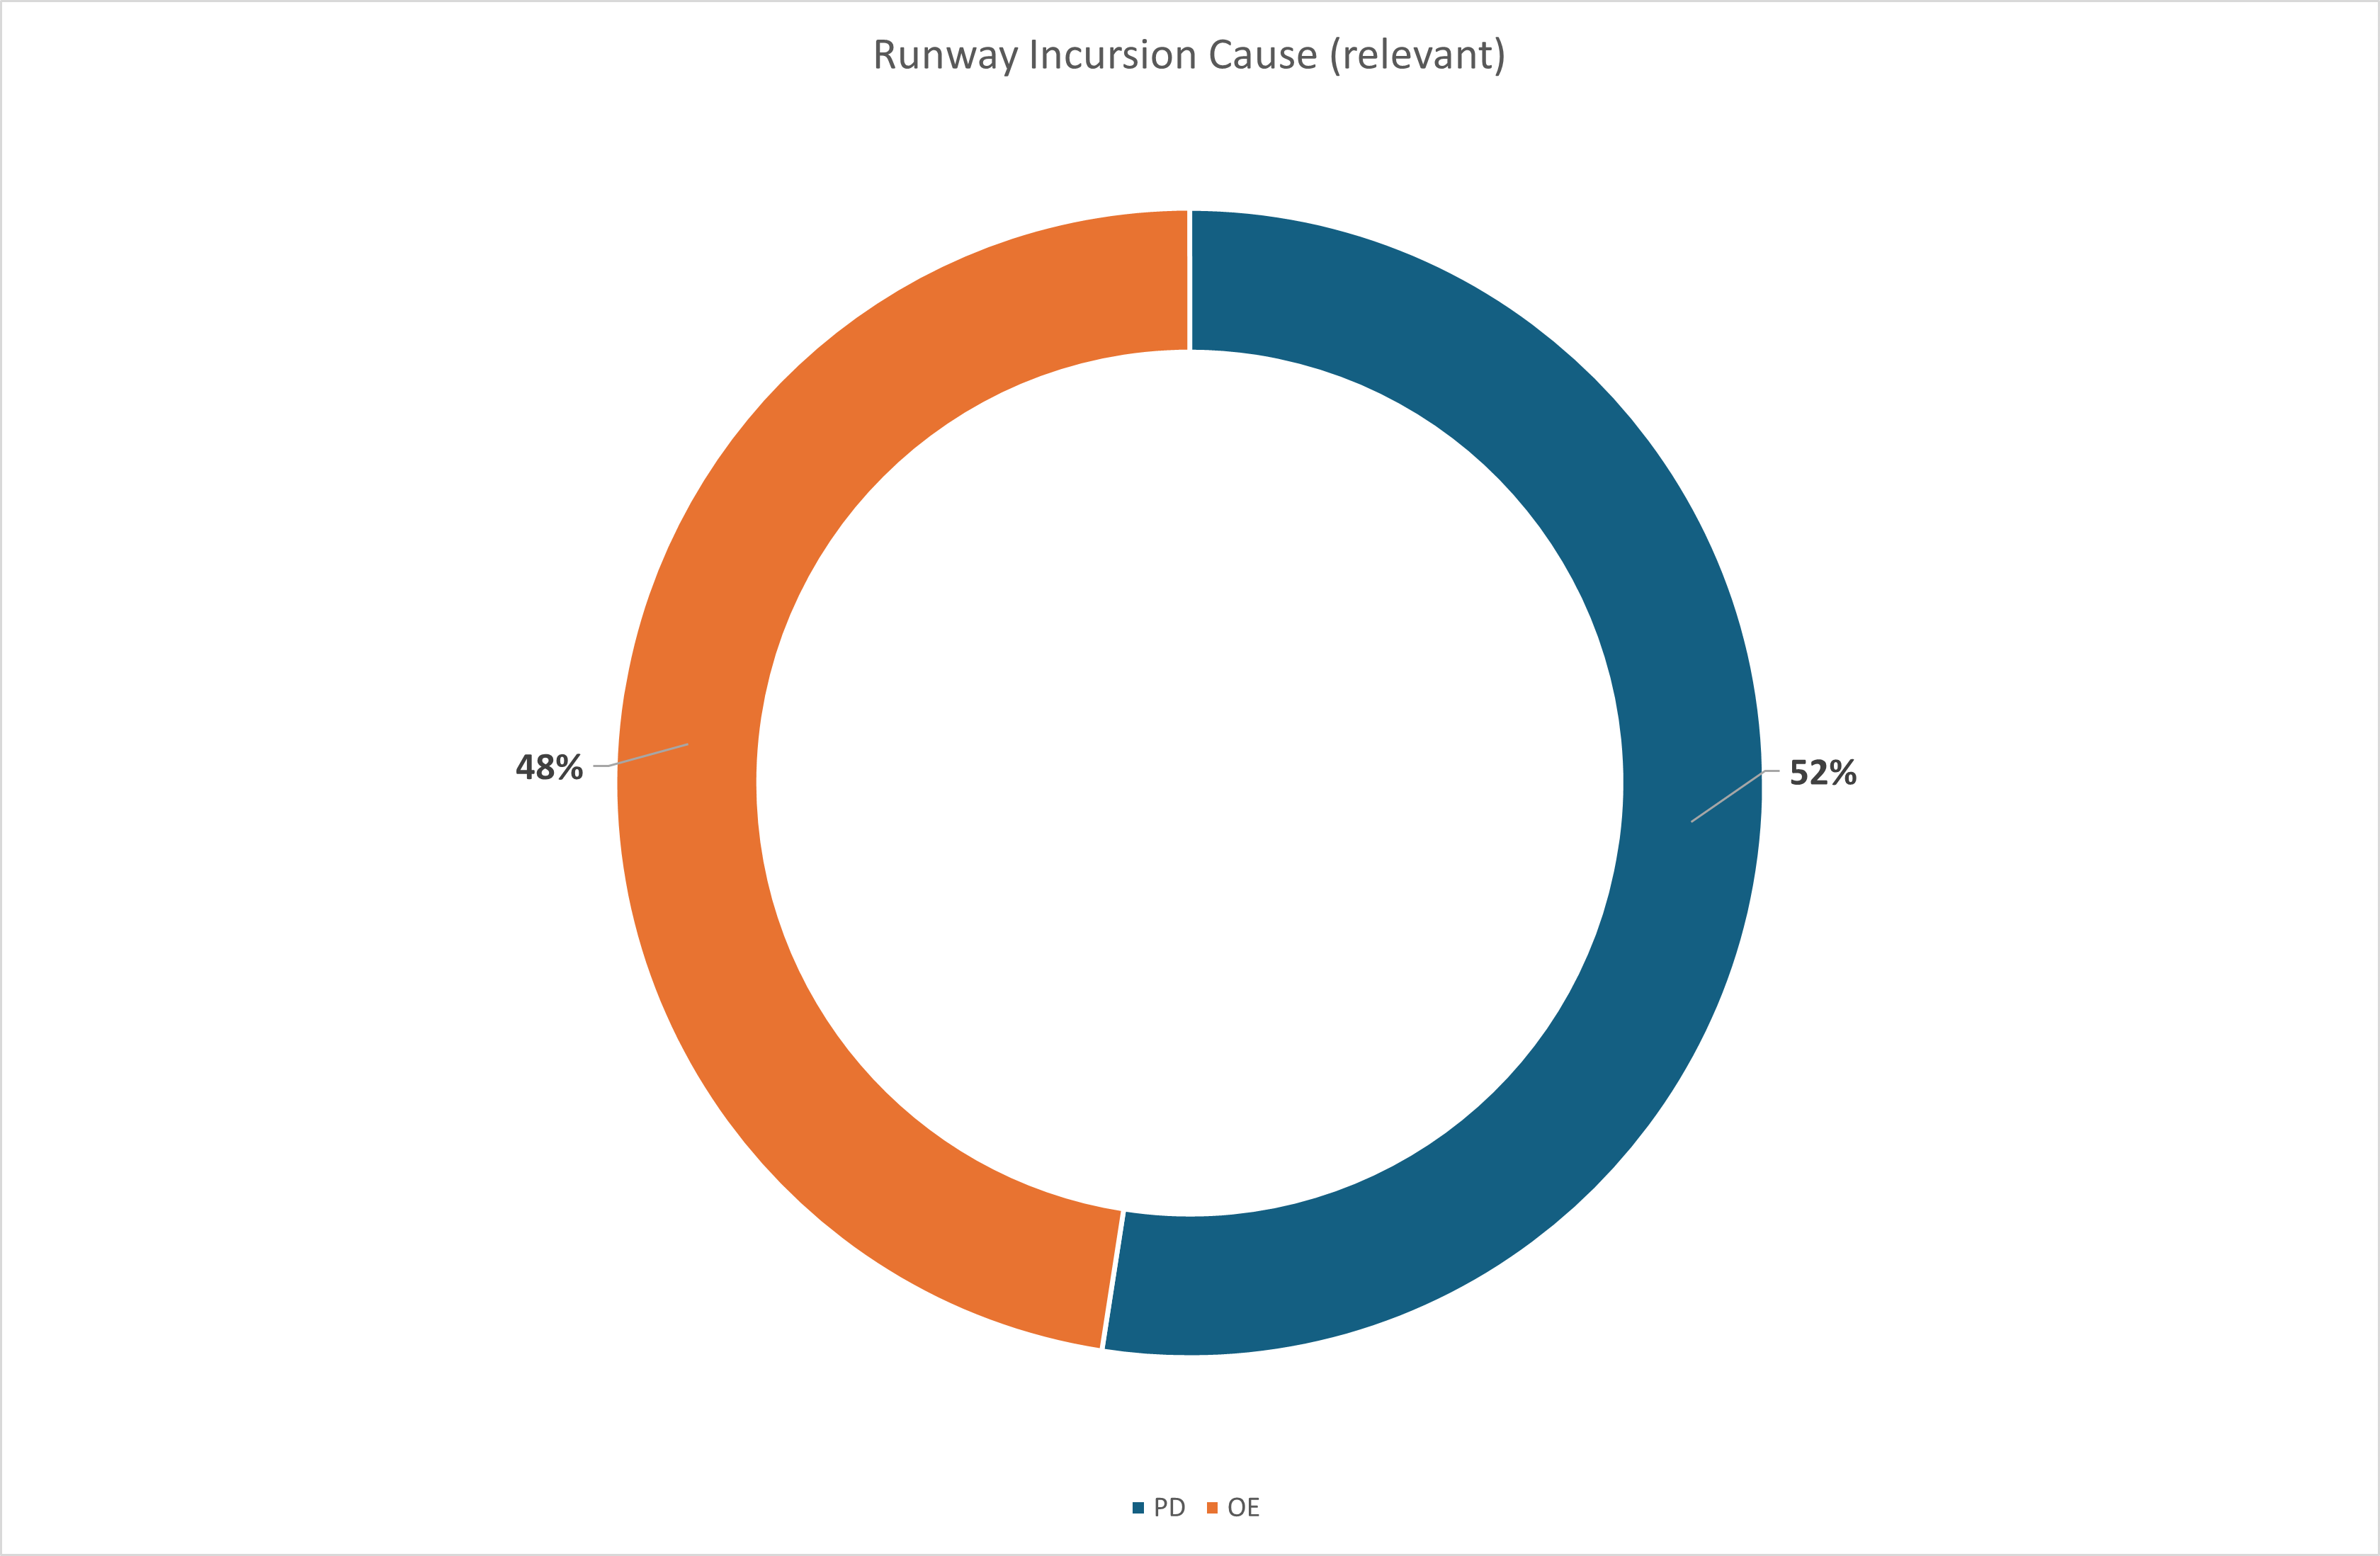
\includegraphics[width=0.75\linewidth]{Abbildungen/Cause_relevant.png}
    \caption{Cause Relevant}
    \label{fig:enter-label}
\end{figure}

\begin{figure} [H]
    \centering
    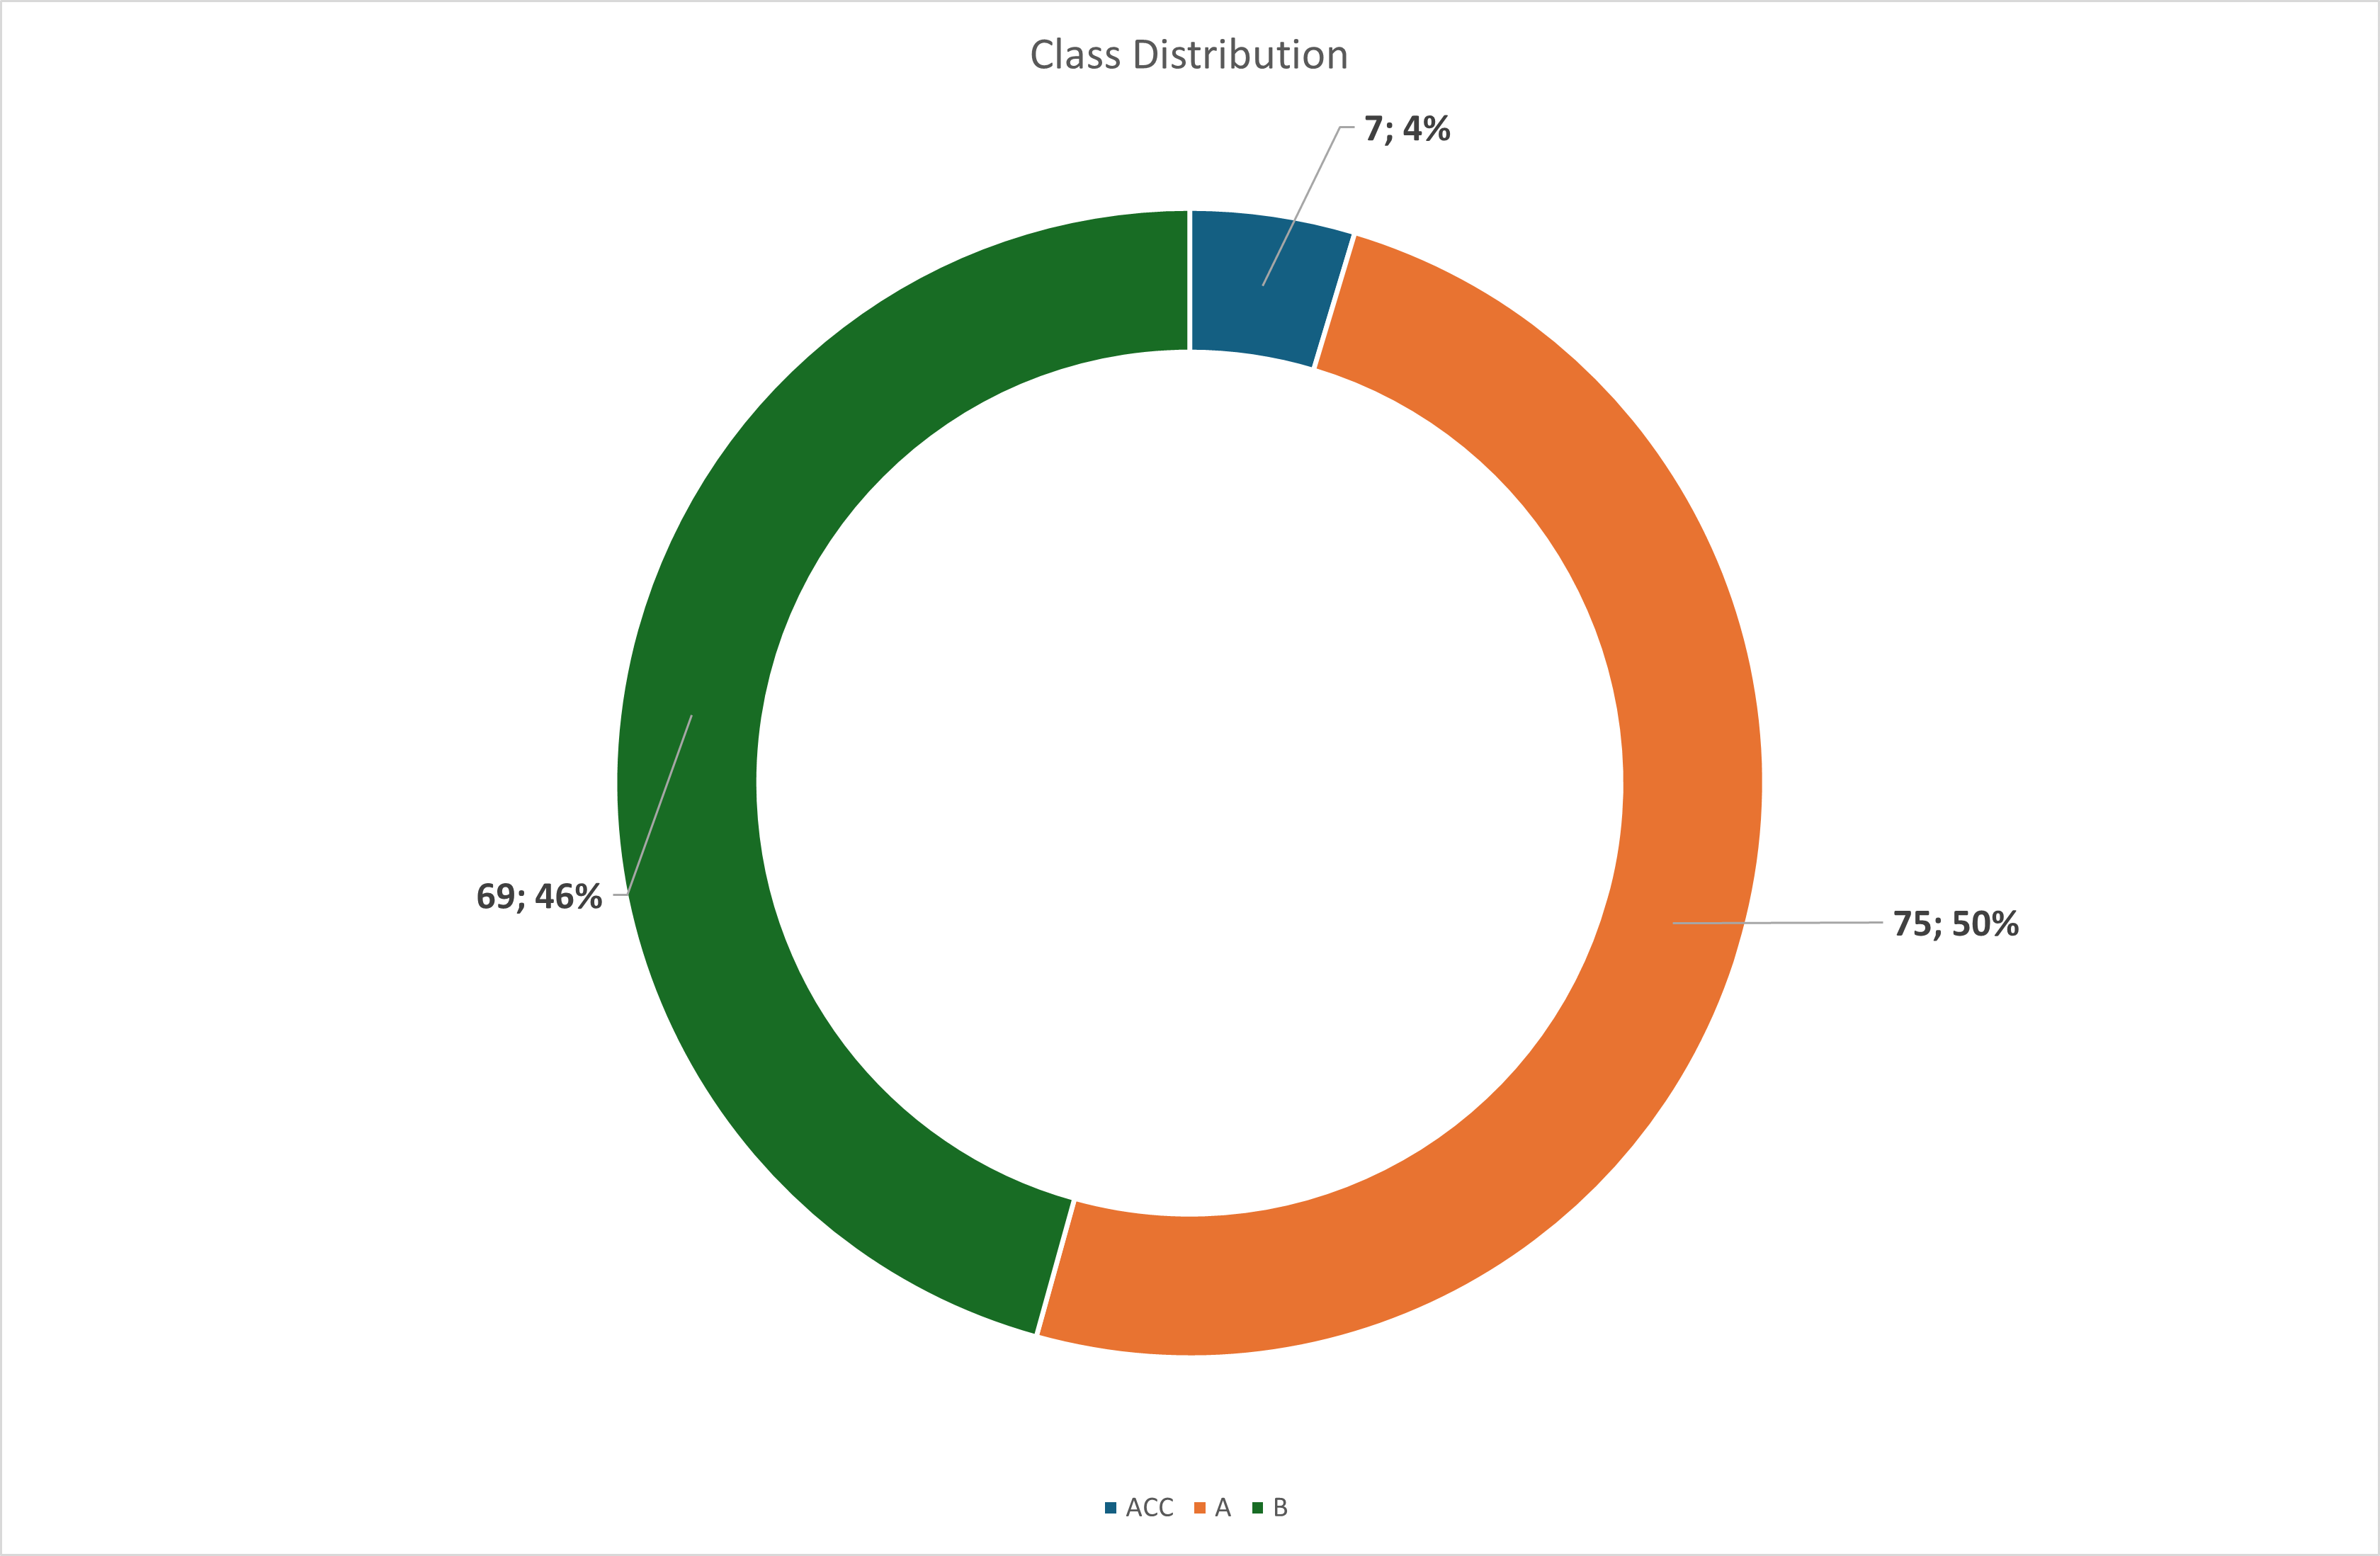
\includegraphics[width=0.75\linewidth]{Abbildungen/Class_relevant.png}
    \caption{Class Distribution}
    \label{fig:enter-label}
\end{figure}

The number of relevant cases was reduced to 192. 151 incidents involving two aircrafts, of which at least one is commercial, and the rest involving one commercial aircraft and a ground vehicle.

\subsection{A and B Runway incursions involving a commercial aircraft}

\begin{figure}[H]
    \centering
    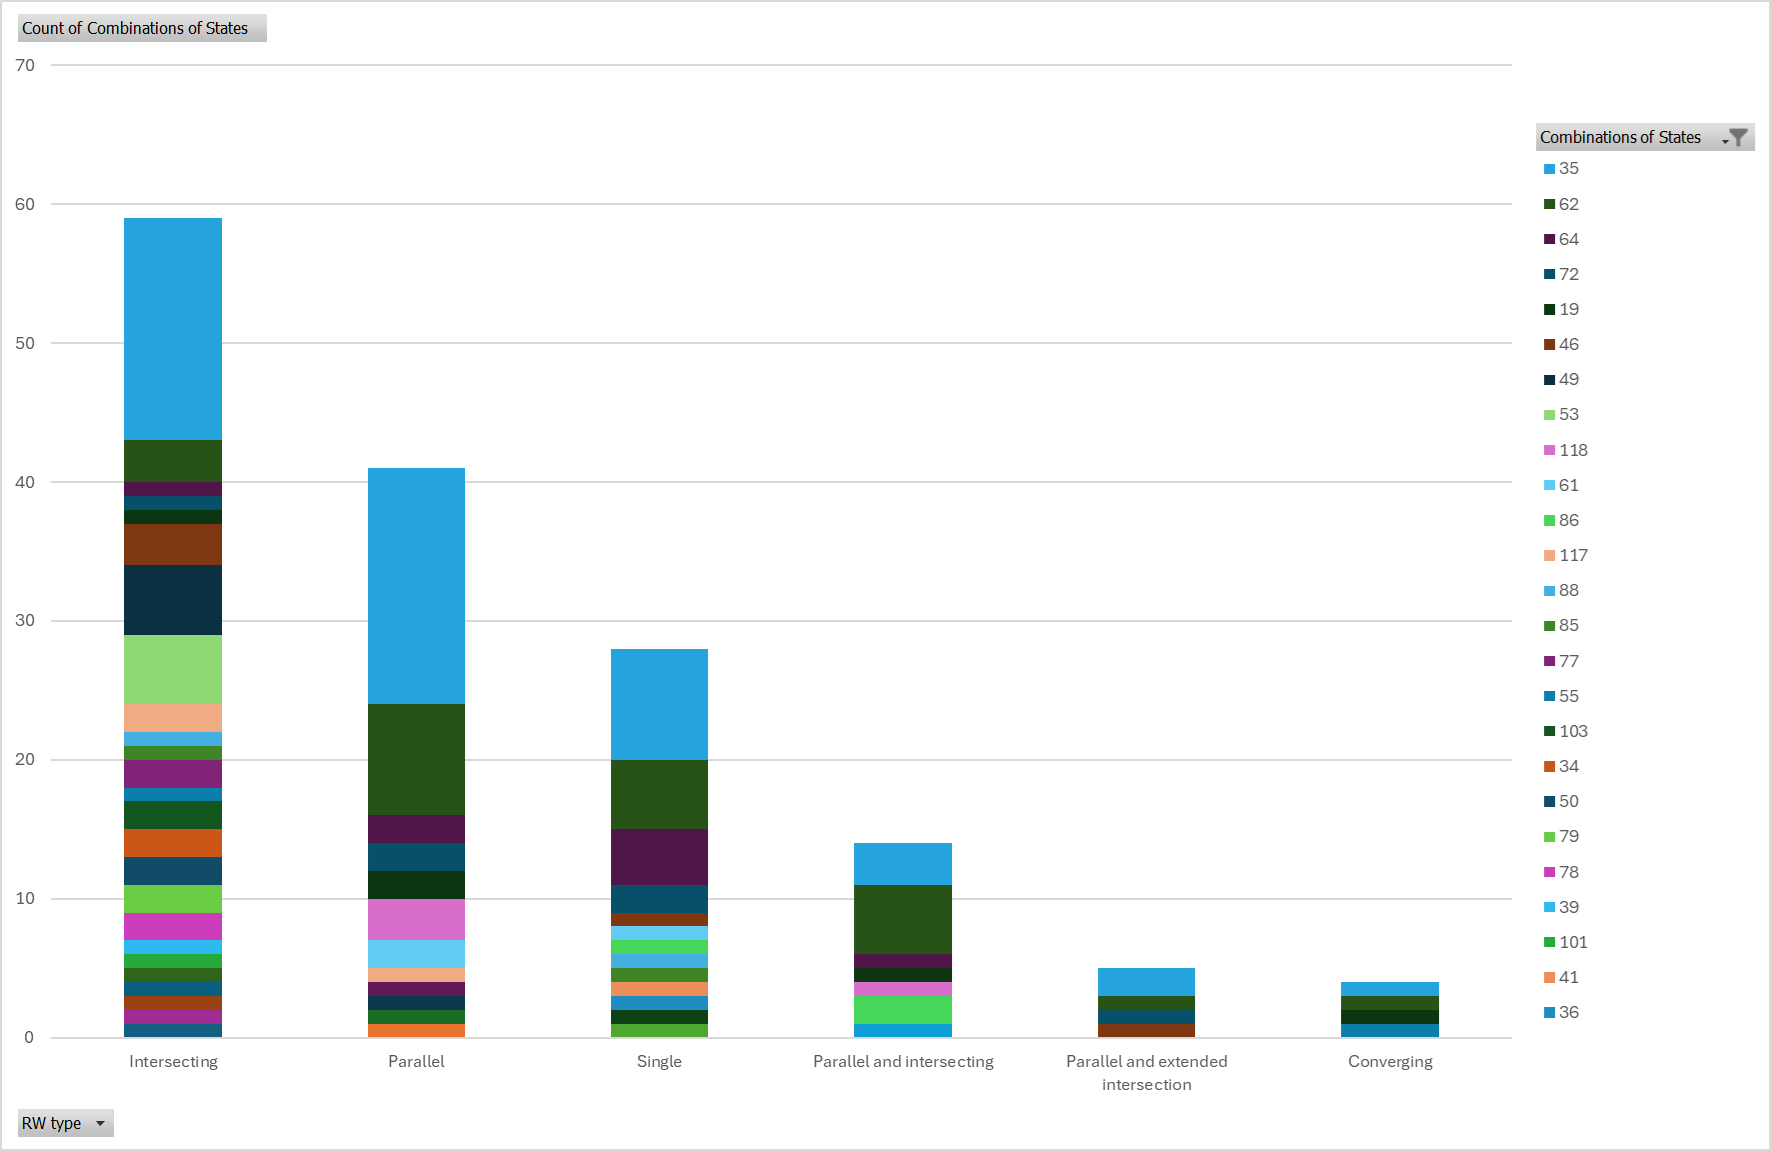
\includegraphics[width = 1\textwidth]{Kapitel/Commercial x other - incursions by runway geometry.png}
    \caption{Count of incidents of A and B Severity involving a commercial aircraft}
    \label{fig:enter-label}
\end{figure}

Figure --- shows the combination of states of the 151 relevant incidents by runway geometry. The runway geometry that has the most incursion cases is the intersecting runway layout, with a total of 59 relevant incidents. It is followed by parallel and single runways, with 41 and 28 incidents respectively. It can be observed that the most common combinations of states are prevalent in every type of runway geometry. 

\begin{table}[H]
\begin{tabular}{cccc}
Combination of   states & Number of runway incursions & ACFT 1 OSED & ACFT 2 OSED \\
35                      & 46                          & III         & II          \\
62                      & 22                          & IV          & II          \\
64                      & 8                           & IV          & III         \\
72                      & 6                           & IV          & VI          \\
46                      & 5                           & III         & VI          \\
49                      & 5                           & III         & IV          \\
53                      & 5                           & III         & III         \\
19                      & 4                           & II          & III         \\
118                     & 4                           & VI          & IV          \\
61                      & 3                           & IV          & I           \\
86                      & 3                           & V           & II          \\
117                     & 3                           & VI          & IV          \\
34                      & 2                           & III         & I           \\
50                      & 2                           & III         & IV          \\
77                      & 2                           & IV          & III         \\
78                      & 2                           & IV          & III         \\
79                      & 2                           & IV          & VI          \\
85                      & 2                           & V           & I           \\
88                      & 2                           & V           & III         \\
103                     & 2                           & V           & III         \\
1                       & 1                           & I           & I           \\
6                       & 1                           & I           & V           \\
21                      & 1                           & II          & IV          \\
36                      & 1                           & III         & II          \\
39                      & 1                           & III         & III         \\
41                      & 1                           & III         & IV          \\
54                      & 1                           & III         & III         \\
55                      & 1                           & III         & VI          \\
56                      & 1                           & III         & VI          \\
74                      & 1                           & IV          & IV          \\
97                      & 1                           & V           & VI          \\
98                      & 1                           & V           & VI          \\
101                     & 1                           & V           & V           \\
111                     & 1                           & VI          & I           \\
112                     & 1                           & VI          & II          \\
116                     & 1                           & VI          & III         \\
130                     & 1                           & VI          & III         \end{tabular}
    \caption{Runway incursions by combination of states} 
\end{table}

Table --- lists the combination of states obtained and the number of incursions that each of those combinations have. combinations of states 35 and 62 are the most common ones, adding up to 68 incursions. 
Those combinations resemble one another in the OSED state of the second aircraft, which is II. this corresponds to events in which the second aircraft enters or crosses the runway while it is being used. If we add combinations 86, 36, and 112, which also involve a second aircraft entering the occupied runway, the number of incursions rises to 73. 


\begin{figure}[H]
    \centering
    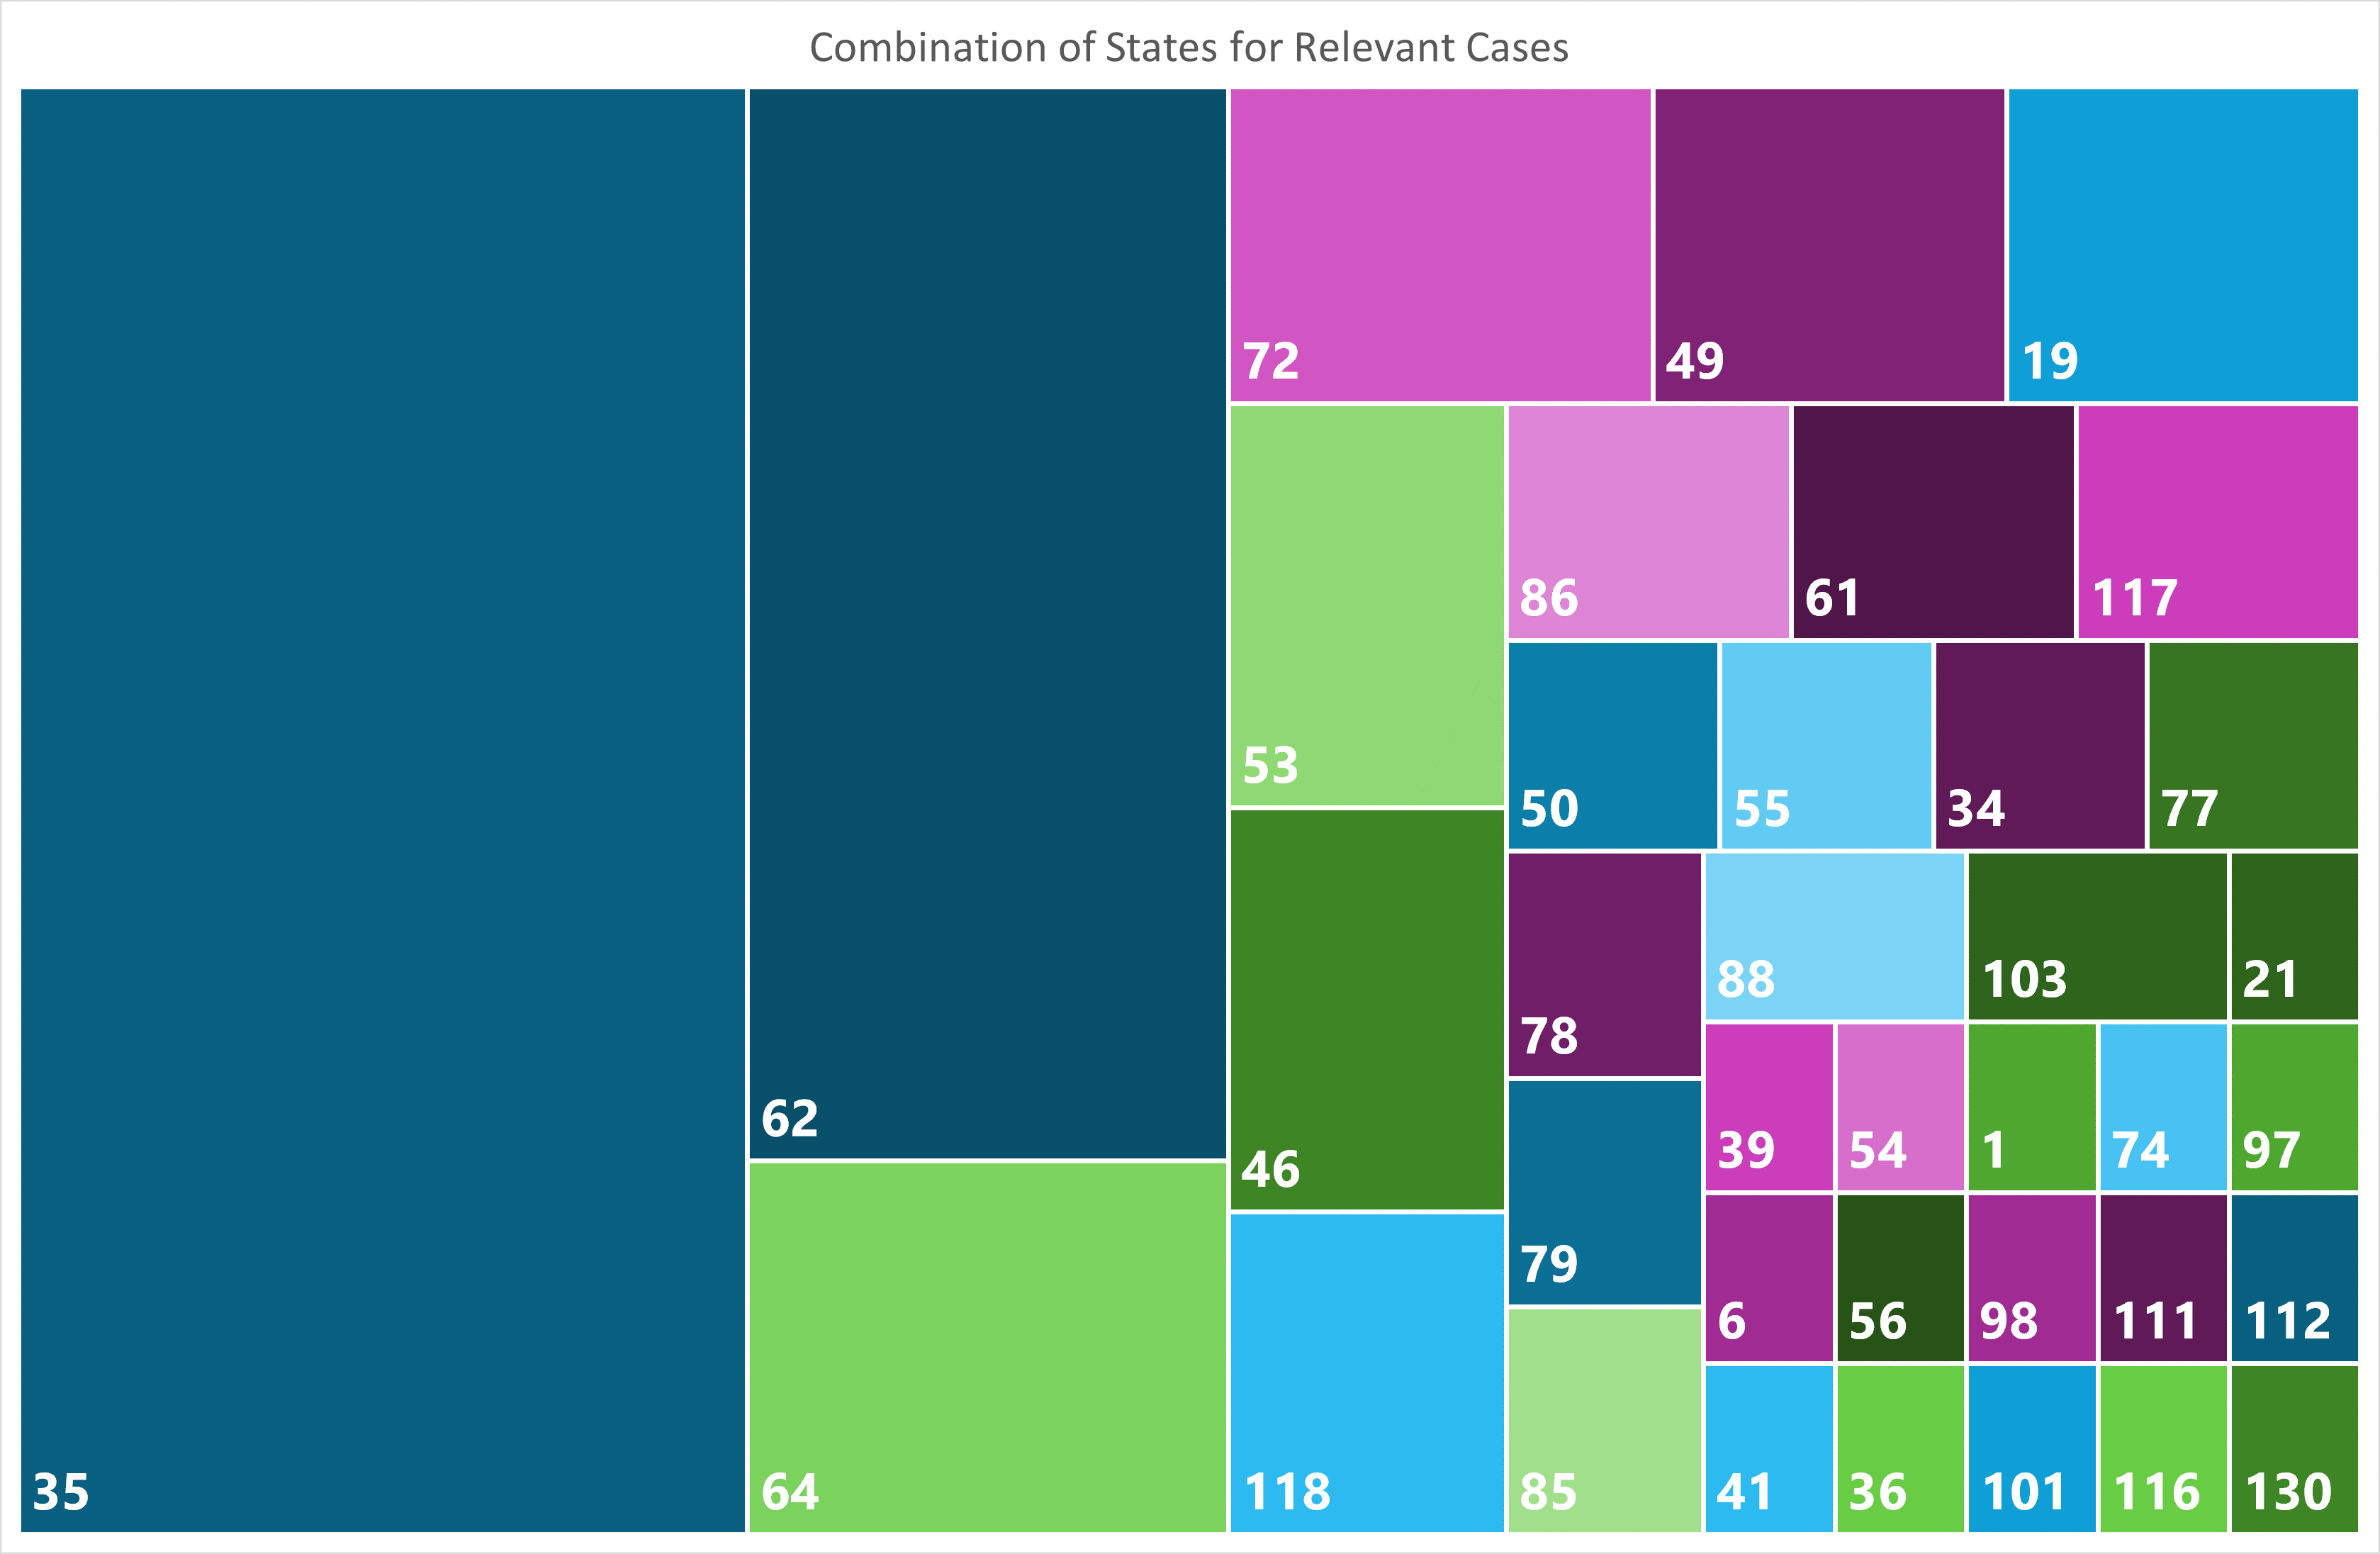
\includegraphics[width = 1\textwidth]{Abbildungen/Combination_of_States.png}
    \caption{Distribution of Combination of states for relevant cases}
\end{figure}

\begin{table}[H]
\begin{tabular}{lcc} 
\multicolumn{1}{c}{Incursion   on} & Combination of   states & Number of   incursions \\ 
Intersecting   runway              & 49                      & 5                      \\ 
Intersecting   runway              & 53                      & 5                      \\ 
Intersecting   runway              & 50                      & 2                      \\ 
Intersecting   runway              & 77                      & 2                      \\ 
Intersecting   runway              & 78                      & 2                      \\ 
Intersecting   runway              & 79                      & 2                      \\ 
Intersecting   runway              & 103                     & 2                      \\ 
Intersecting   runway              & 54                      & 1                      \\ 
Intersecting   runway              & 55                      & 1                      \\ 
Intersecting   runway              & 56                      & 1                      \\ 
Intersecting   runway              & 74                      & 1                      \\ 
Intersecting   runway              & 101                     & 1                      \\ 
Intersecting   runway              & 130                     & 1                      \\ 
Intersecting   runway              & Total                   & 26                     \\ 
Single runway                      & 35                      & 16                     \\ 
Single runway                      & 62                      & 3                      \\ 
Single runway                      & 64                      & 1                      \\ 
Single runway                      & 72                      & 1                      \\ 
Single runway                      & 46                      & 3                      \\ 
Single runway                      & 19                      & 1                      \\ 
Single runway                      & 117                     & 2                      \\ 
Single runway                      & 34                      & 2                      \\ 
Single runway                      & 85                      & 1                      \\ 
Single runway                      & 88                      & 1                      \\ 
Single runway                      & 39                      & 1                      \\ 
Single runway                      & 116                     & 1                      \\ 
                                   & Total                   & 33                     \\ 
\end{tabular}
\caption{Combination of states on intersecting runways}
\end{table}

Taking a closer look at the incursions that occurred on intersecting runways shown on table ---, it can be observed that out of the 59 incursions, 26 correspond to runway incursions that took place on intersecting runways, while 33 of them did not involve the intersecting runway. The incursions involving the intersecting runway appear to be significant, as they account for almost half of the incursions on these runways. This is consistent with what would be expected, as an intersecting runway adds to the complexity of the layout. It introduces combinations of OSED states that correspond to incursions that are not possible on single or parallel runways.  

\subsection{A and B Runway incursions involving a commercial aircraft and a ground vehicle}

\begin{figure}[H]
    \centering
    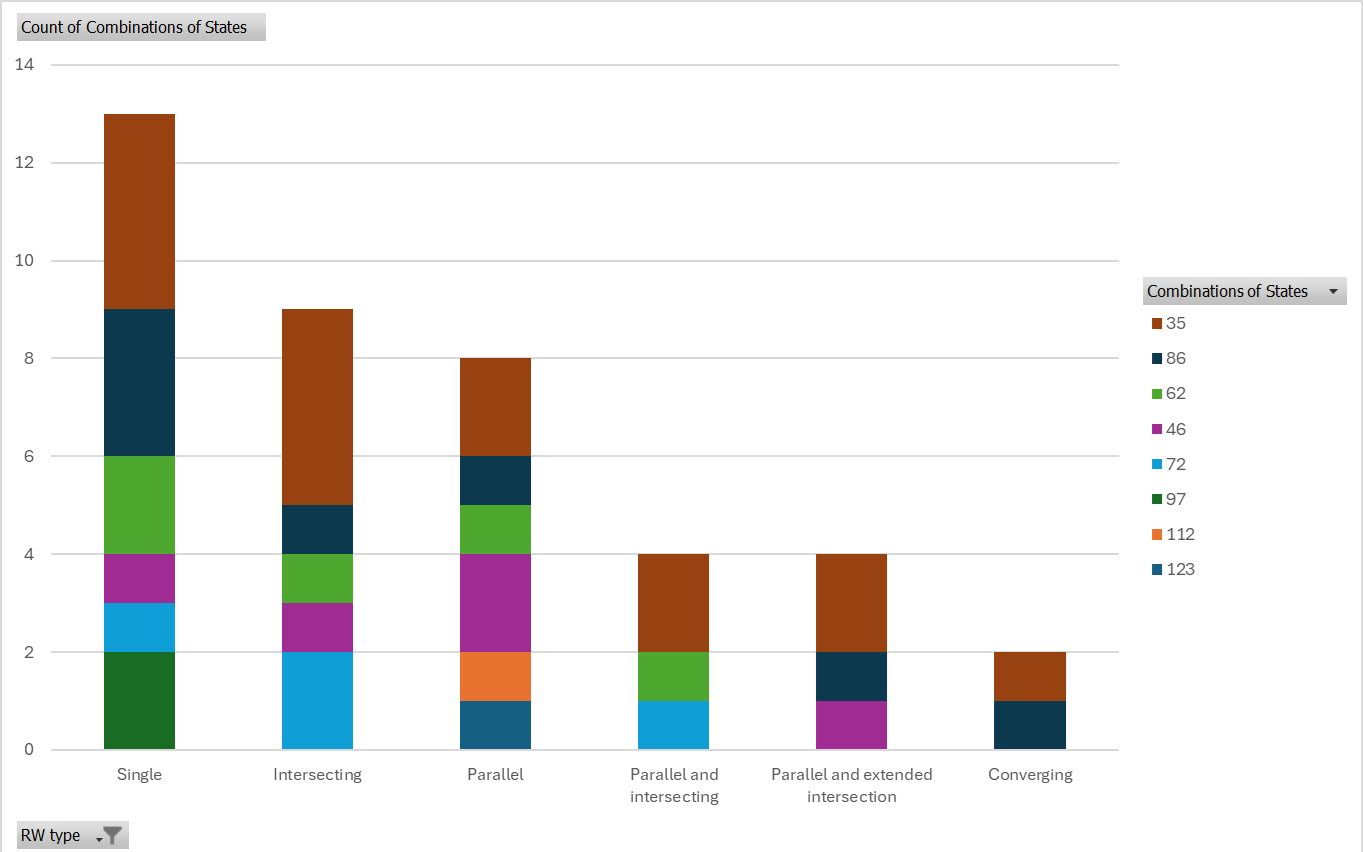
\includegraphics[width = 0.8\textwidth]{Kapitel/Commercial x ground vehicle - incursions by geometry.png}
    \caption{Count of incidents of A and B Severity involving a commercial aircraft and a ground vehicle}
    \label{fig:enter-label}
\end{figure}

Figure --- shows the combination of states by runway geometry of the 40 incursions involving a commercial aircraft and a ground vehicle. Contrary to the incidents involving two aircrafts, the most common runway geometry in this case is single runways, followed by intersecting and parallel runways. This is to be expected as even though intersecting runways add complexity, it is unlikely that a vehicle will be taxiing in a runway, they mostly just cross them unless they are doing surveillance or maintenance activities. All of the 40 incidents are a single runway incursions. 